
\documentclass[a4paper,twoside,openright,12pt,Slovene]{book}
\usepackage[pdftex]{UNI-LJ-FE-Diploma} % stil zaključnega dela UL FE
\usepackage[utf8]{inputenc} % predloga uporablja standardno kodiranje Unicode UTF-8, ki podpira šumnike
\usepackage[greek,english,Slovene]{babel} % seznam uporabljenih jezikov (zadnji na seznamu je primarni)


\usepackage{filecontents}
\begin{filecontents*}{\jobname.xmpdata}
    \Title{Simulator elektrostatične raztelektritve} % Mora biti enak kot je v prijavi teme!
    \Author{Vid Oblak} % Mora biti enak kot na naslovnici!
\end{filecontents*}
\usepackage[a-1b]{pdfx}
%%%%%%%%%%%%%%%%%%%%%%%%%%%%%%%%%%%%%%%%%%%%%%%%%%%%%%%%%%%%%%%%%%%%%%%%%%%%%%%%%%%%%%%%%%%%%%%%%%%%%%%%%%%%%%%%%%%%%%%%


% Kompakten pregled LaTeX ukazov je dostopen na https://en.wikibooks.org/wiki/Category:Book:LaTeX
% Navodila posameznih uporabljenih paketov so dostopna na https://www.ctan.org

% Dodatni simboli
\usepackage{textcomp}                               % dodatni simboli (kot npr. €)
\usepackage{gensymb}                                % dodatni simboli \de­gree, \cel­sius, \pert­hou­sand, \mi­cro, \ohm
\newcommand{\uppi}{\textrm{\greektext p\latintext}} % velika grška črka P z \uppi, alternativa simbolu \Pi

% Osnovno oblikovanje
\hypersetup{unicode,hidelinks,breaklinks,hyperindex} % dodatne možnosti hiperpovezav
\usepackage[normalem]{ulem}                          % podčrtavanje in prečrtavanje teksta
\usepackage{float}                                   % dodatne možnosti oblikovanja objektov
\usepackage{enumitem}                                % dodatne možnosti oblikovanja seznamov

% Dodatno oblikovanje
%\zamaknirobsodihstrani{0mm} % dodatna prilagoditev levega roba sodih strani za dvostranski tisk
%\usepackage{dcolumn}        % poravnava po decimalnih mestih v tabelah
%\usepackage{longtable}      % večstranske tabele
%\usepackage{caption}        % dodatne možnosti označevanja objektov
%\usepackage{rotating}       % vretenje objektov, strani, ipd.

\usepackage{siunitx} %uporaba SI simbolov

% Matematična orodja
\usepackage{mathtools} % http://mirrors.ctan.org/macros/LaTeX/contrib/mathtools/mathtools.pdf
\usepackage{bm}        % ukaz za odebeljeni tisk \bm v matematičnih okoljih
%\usepackage{cancel}   % ukaz za prečrtavanje \cancel v matematičnih okoljih

% Grafična orodja
\usepackage{graphicx}                 % vključevanje bitnih slik z ukazom \includegraphics
\usepackage{grffile}                  % podpora presledkom pri ukazu \includegraphics
%\usepackage{tikz}                    % paket TikZ za risanje (npr. blokovnih shem, diagramov poteka, itd.)
%\usetikzlibrary{calc,shapes,arrows}  % dodatne možnosti paketa TikZ
%\usepackage{tikzscale}               % skaliranje risb
\usepackage[smartlabels, european, americaninductors]{circuitikz} % risanje shem vezij
%\usepackage{pgfplots}                % paket PGFPlots za risanje grafov, tudi iz CSV in podobnih datotek
%\usepgfplotslibrary{polar,external}  % dodatne možnosti paketa PGFPlots
%\usepackage{tikz-3dplot}             % 3D risanje
% Primeri: http://texample.net , http://pgfplots.net/tikz/examples , http://pgfplots.sourceforge.net/gallery.html

% Vključevanje datotek
\usepackage{pdfpages} % vključevanje PDF datotek z ukazom \includegraphics
\usepackage{epstopdf} % vključevanje EPS datotek z ukazom \includegraphics
\usepackage{listings} % orodja za izpisovanje programske kode
\lstset{              % nastavitve orodja za izpisovanje programske kode
    basicstyle=\ttfamily\footnotesize,
    breaklines=true,
    numbers=left,
    numberstyle=\scriptsize,
    keywordstyle=\color{blue},
    commentstyle=\color{unilj},
    stringstyle=\color{olive},
}
%%%%%%%%%%%%%%%%%%%%%%%%%%%%%%%%%%%%%%%%%%%%%%%%%%%%%%%%%%%%%%%%%%%%%%%%%%%%%%%%%%%%%%%%%%%%%%%%%%%%%%%%%%%%%%%%%%%%%%%%

% DEKLARACIJE %%%%%%%%%%%%%%%%%%%%%%%%%%%%%%%%%%%%%%%%%%%%%%%%%%%%%%%%%%%%%%%%%%%%%%%%%%%%%%%%%%%%%%%%%%%%%%%%%%%%%%%%%%
\naslov{Simulator elektrostatične razelektritve} % Mora biti enak kot je v prijavi teme!
\avtor{Vid Oblak} % Mora se ujemati s \Title pri metapodatkih PDF/A!
\mentor{Izr. Prof. Dr. Peter Zajec}
%\somentor{Naziv, ime in priimek somentorja}
\date{Ljubljana, \the\year}
\univerza{Univerza v Ljubljani}
\definecolor{unilj}{cmyk}{0.00, 0.94, 0.94, 0.06} % barva Univerze v Ljubljani

\delo{Poročilo o delu\\~\\Visokošolski strokovni študijski program\\prve stopnje Aplikativna elektrotehnika}
\fakulteta{Fakulteta za elektrotehniko}

% DOKUMENT %%%%%%%%%%%%%%%%%%%%%%%%%%%%%%%%%%%%%%%%%%%%%%%%%%%%%%%%%%%%%%%%%%%%%%%%%%%%%%%%%%%%%%%%%%%%%%%%%%%%%%%%%%%%%
\begin{document}

\frontmatter

\selectlanguage{slovene}

%******************************* NASLOVNICA ************************************
\maketitle

%******************************* ZAHVALA ***************************************
\zahvala
Zahvaljujem se mentorju dr. Petru Zajcu in mentorju v podjetju Blažu Prahu, katera sta mi pomagala z nasveti, izračuni in realizacijo projekta. Zahvaljujem se tudi sodelavcu Janu Pogačarju, kateri mi je vskočil na pomoč pri uporabi Python in LaTeX. Prav tako se zahvaljujem vsem ostalim sodelavcem in prijateljem, kateri so tudi v najmanjši meri pomagali pri razvoju ali realizaciji projekta.


%******************************* POVZETEK IN KLJUČNE BESEDE ********************
\povzetek
V tem zaključnem poročilu je opisan razvoj simulatorja elektrostatične razelektritve za integrirana vezja in problemi, ki sem jih imel pri razvoju. Simulator je sestavljen iz treh glavnih modulov in sicer kontrolne ploščice, nastavljivega visokonapetostnega napajalnika in visokonapetostnega stikala.
Zaradi trenutne gospodarske situacije smo se tekom razvoja projekta odločili da bomo dali poudarek na ugodni ceni. Ta zahteva je pomenila razvoj in izdelavo nastavljivega visokonapetostnega napajalnika in visokonapetostnega stikala, namesto nakupa le teh. 
Vsi moduli projekta so bili načrtovani z modularnostjo v mislih, da v primeru kasnejše nadgradnje ali zamenjave ta poteka čim bolj nemoteno. Vendar sem tekom projekta sem ugotovil, da bi izdelava simulatorja kateri bi ustrezal vsem standardom bi zahtevala precej več časa in večji proračun.

\kljucnebesede
ESD, Elektrostatika, Simulator elektrostatične razelektritve, mikroelektronika

\selectlanguage{english}

%******************************* ABSTRACT AND KEYWORDS *************************

\abstract
In this final report is description of development of ESD simulator for microelectronics and problems which I experienced within development. Simulator is made of three main modules: main control board, adjustable high-voltage power supply and high-voltage switch. Due to current economy situation we have decided to put emphasis on low-cost of the simulator. This meant development and manufacturing of our own adjustable high-voltage power supply and high-voltage switch, instead of purchasing. All modules of the simulator were designed to be modular and swappable, that way upgrades or replacements can be made without major disruption. But during development I have come to conclusion that ESD simulator which would fit the requirements can not be made in specified time frame and with current budget.

\keywords
ESD, Electrostatic, ESD Simulator, microelectronics

\selectlanguage{slovene}

%******************************* KAZALO ****************************************
\tableofcontents

%******************************* SEZNAM SLIK, SEZNAM TABEL *********************
\seznamslik
\seznamtabel

%******************************* SEZNAM SIMBOLOV *******************************
\seznamsimbolov
V pričujočem zaključnem delu, so uporabljene naslednje veličine in simboli:

\begin{center}
    \begin{tabular}{*{4}{l}} \hline
        \multicolumn{2}{c}{\bf{Veličina / oznaka}}           & \multicolumn{2}{c}{\bf{Enota}} \\ \hline
        Ime                & Simbol                          & Ime      & Simbol              \\ \hline
        čas                & $t$                             & sekunda  & s                   \\
        frekvenca          & $f$                             & Hertz    & Hz                  \\
        napetost           & $U$                             & Volt     & V                  \\
        tok                & $I$                             & Amper    & A                   \\
        upornost           & $R$                             & Ohm      & $\Omega$            \\ \hline

    \end{tabular}
\end{center}

Natančnejši pomen simbolov ter njihovih indeksov je razviden iz ustreznih slik ali pa je pojasnjen v spremljajočem besedilu, kjer je simbol uporabljen.

\mainmatter

%******************************* UVOD ******************************************
\chapter{Uvod} \label{uvod}

Praktično usposabljanje sem opravljal v podjetju Renishaw d.o.o.  Podjetje se ukvarja z integriranimi vezji za specifično uporabo (ASIC) in je bilo ustanovljeno leta 2014 kot hčerinsko podjetje Britanskega podjetja Renisahw p.l.c. Zaposleni so razdeljeni na tri skupine:
\begin{itemize}
	\item Načrtovalci: načrtujejo posamezne sklope integriranega vezja in karakterizirajo vezje s pomočjo simulacij.
	\item Oblikovalci sestavnice mask: postavijo posamezne komponente na površino integriranega vezja (podobno kot risanje tiskanih vezij).
	\item Testni inženirji: karakterizirajo narejena integrirana vezja, načrtujejo testna vezja in skrbijo za testiranje vezij za proizvodnjo.
\end{itemize}
Sam sem izvajal praktično usposabljanje v skupini testnih inženirjev. Pod to skupino delam v tem podjetju že 3 leta, zaradi tega so mi bile poznane že vse procedure in sem se lahko takoj lotil naloge. Zadana mi je bila naloga zasnove in izdelave simulatorja elektrostatične razelektritve, kateri se uporablja pri verifikaciji integriranih vezij. Zahteve so bile po maksimalni napetosti vsaj \SI{15}{\kilo\volt} DC, nastavljivost izhodne napetosti med \SI{250}{\volt} in \SI{15}{\kilo\volt}, natančnost izhodne napetosti vsaj 3\% ter ustrezanje CE zakonodaji. 

\begin{figure}[H]
	\centering
    \begin{circuitikz}
        \draw (0,0)
       to[V, v=$V$] (0,3)
       to[R=1M] (2,3)
       to[short] (2.685,3)
       to[short] (2.685,2.5);
       
       \draw (3,2)
       node[spdt, rotate=90] {};
       
       \draw (0,0)
       to[short] (3,0)
       to[C=100pF] (3,1.5);
       
       \draw (3,0)
       to[short] (5,0)
       to[short, -d] (5,0.5);
       
       \draw (3.315,2.5)
       to[short] (3.315,3)
       to[R=1500Ohm] (5,3)
       to[short, -d] (5,2.5);
    \end{circuitikz}
          \caption{\label{ESDTesterShemaOsnovna} Osnovna shema ESD simulatorja.}
    \end{figure}

Za potrebe testiranja integriranih vezij smo v podjetju potrebovali simulator elektrostatične razelektritve. Na začetku snovanja so bile zastavljene specifikacije maksimalne napetosti \SI{15}{\kilo\volt} in uporaba že narejenih modulov za nastavljivi visokonapetostni napajalnik ter visokonapetostno stikalo. Tekom projekta se je to spremenilo in prišlo do odločitve o lastnem načrtovanju nastavljivega visokonapetostnega napajalnika. Pri tem modulu sem imel za prebresti kar nekaj tehničnih ovir. Največji sta bili ustrezanje regulacijam CE ter zagotavljanje \SI{15}{\kilo\volt} izolacije med primarno in sekundarno stranjo.   
Princip delovanja simulatorja elektrostatične razelektritve je dokaj enostaven. Nastavljivi visokonapetostni vir polni kondenzator, katerega se nato preko upora prazni skozi testiranec.    
Prvotni načrti so bili lastno navijanje primernega visokonapetostnega transformatorja. Po kar nekaj meritvah in izračunih se je to pokazalo za neprimerno, saj nismo uspeli zagotoviti željene napetosti in izolacije. Rezervni načrt je bil razdreti televizor s katodno cevjo in iz tam vzeti ven transformator. Temu smo se hoteli izogniti saj se že trenutno težko najde televizorje s katodno cevjo, čez leta se jih bo pa še težje. Motilo me je pa tudi razlikovanje transformatorjev tako v podnožju kot v karakteristikah in vgrajene diode v sekundarnem navitju še dodatno otežijo karakterizacijo transformatorja. 
Regulacija napetosti nam je povzročala probleme zaradi zagotavljanja željene izolacije. S pomočjo simulacij sem preizkusil kateri tipi napetostnih krmilnikov bi nam ustrezali. Izločili smo vse neizolirane krmilnike. Krmilnik s povratno vezavo preko optičnega spojnika ni zmožen pokrivati celotne izhodne napetosti od \SI{250}{\volt} do \SI{15}{\kilo\volt}, zaradi nelinearnosti optičnega krmilnika, krmilnik s povratno vezavo preko pomožnega navitja je v simulacijah zdel obetavno, vendar se je na koncu izkazal za neprimernega. Kot primeren se je izkazal samo regulator, ki ima povratno vezavo preko primarnega navitja in sicer z merjenjem zrcaljene napetosti z sekundarnega navitja na primarno. Po obsežnejših meritvah pa nas je tudi ta razočaral. Na koncu smo naredili regulator z mikrokrmilnikom, kateri prejema povratno vezavo preko galvansko ločenega analogno-digitalnega pretvornika.
Po standardih MIL-STD-883K ~\cite{MIL-STD-883K} in JS-001-2007 ~\cite{JS-001-2017} mora biti visokonapetostno stikalo, katero prazni kondenzator skozi testiranec t.i. ''bounce-less'', se pravi ko sklene kontakt ga mora zadržati, namesto, da ga na kratko večkrat razklene in sklene. Standarda pa tudi predpisujeta obliko signala toka skozi testiranec, zato razbremenilno vezje t.i. ''snubber'' čez kontakte stikala ni primerna rešitev. Za nižje napetosti obstajajo releji, kateri vsebujejo živo srebro, čigar naloga je zadržati kontakt, ko se kontakta odbijeta. Vendar cena takšnega releja za \SI{15}{\kilo\volt} znaša okoli \texteuro2000.
Kompromis je bil izdelava svojega stikala, katero bo ustrezalo zahtevam.





%******************************* POGLAVJA **************************************
\chapter{Simulator elektrostatične razelektritve} \label{ESDSIM}

	\section{Praktično usposabljanje}
	Načrtovalski del projekta, sem delal na svojem računalniškem delovnem mestu, kjer sem uporabljal:
	\begin{itemize}
		\item Altium Designer: risanje električnih shem in načrtovanje tiskanih vezij.
		\item Visio: risanje blok diagramov in konceptnih shem.
		\item LTSpice: simulacija analognih vezij.
		\item STM32Cube: programiranje mikrokrmilnikov ARM STM32.
		\item Python: komunikacija med mikrokrmilnikom in računalnikom.
	\end{itemize}
	Na svoji delovni mizi sem imel antistatično podlogo, vendar to delovno mesto ni bilo namenjeno meritvam, morda samo hitrim meritvam, s katerimi sem potrdil koncept.
	Za obsežnejše meritve sem imel na voljo merilno mesto, kjer je bilo tudi na voljo več merilnih inštrumentov. Pri svojem delu sem največ uporabljal:
	\begin{itemize}
		\item Rigol DS1054Z: digitalni osciloskop.
		\item Acute ADP2100 : visokonapetostna diferencialna sonda.
		\item Rigol DP832: 3 kanalni laboratorijski napajalnik.
		\item PeackTech 3450: multimeter z vgrajeno termalno kamero.
	\end{itemize}
	Pred delom z visoko napetostjo je bilo potrebno opraviti interni tečaj varstva pri delu z visoko napetostjo. Po posvetu z mentorjem, sva sklenila razdeliti nalogo po posameznih modulih. Za vsak modul sem naprej pripravil blokovno shemo, ter opis možnih rešitev, po pregledu le teh je sledilo nadaljnje simuliranje v LTSpice in ko smo bili zadovoljni z rezultati še načrtovanje v Altium Designer.
	
	\section{Zasnova simulatorja elektrostatične razelektritve}
	Poleg že omenjenih specifikacij je veljalo tudi, da mora simulator ustrezati standardoma MIL-STD-883K in JS-001-2007. Osnovna shema simulatorja je sledeča:
	\begin{figure}[h]
	\centering
    \begin{circuitikz}
        \draw (0,0)
       to[V, v=$V$] (0,3)
       to[R=1M] (2,3)
       to[short] (2.685,3)
       to[short] (2.685,2.5);
       
       \draw (3,2)
       node[spdt, rotate=90] {};
       
       \draw (0,0)
       to[short] (3,0)
       to[C=100pF] (3,1.5);
       
       \draw (3,0)
       to[short] (5,0)
       to[short, -d] (5,0.5);
       
       \draw (3.315,2.5)
       to[short] (3.315,3)
       to[R=1500Ohm] (5,3)
       to[short, -d] (5,2.5);
    \end{circuitikz}
          \caption{\label{ESDTesterShemaOsnovna} Osnovna shema ESD simulatorja.}
    \end{figure}
    
	Sestavljajo ga nastavljivi visokonapetostni izvir, polnilni upor, praznilni kondenzator, praznilni upor ter ne-preskakovalno (t.i. bounce-less) stikalo. Preko polnilnega upora se napolni praznilni kondenzator na željeno napetost, katerega se preko praznilnega upora sprazni skozi testiranec. Izhodni tok mora ustrezati limitam, katere so podane v standardih: dvižni čas mora biti manjši kot \SI{10}{\nano\second} ter nominalni čas praznjenja kondenzatorja skozi kratek stik mora biti \SI{150}{\nano\second}, z maksimalnim odstopanjem \SI{\pm 20}{\nano\second}. Slednja zahteva pomeni, da s stikalom, povezovalnimi žicami in konektorji smemo dodati maksimalno \SI{20}{\pico\farad} parazitne kapacitivnosti, saj drugače bo čas izpraznitve skozi kratek stik odstopal zahtevanemu. Pri načrtovanju visokonapetostnega izvira je prav tako potrebno biti previden, saj mora zagotavljati \SI{15}{\kilo\volt} izolacije med primarno in sekundarno stranjo.
%diplomska - slika grafa iz standarda

	\subsection{Moduli simulatorja}
	Simulator je sestavljen iz 4 modulov, od katerih vsak opravlja posebno nalogo.
	\begin{figure}[h]
    \centering
    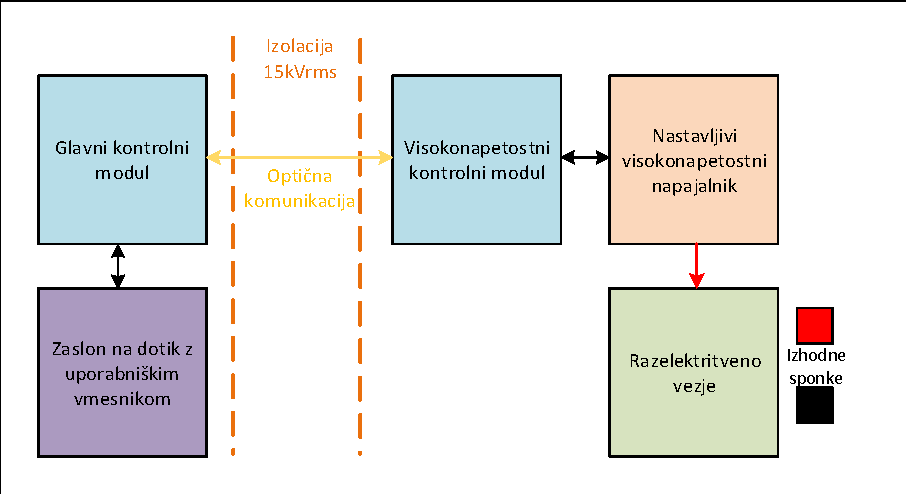
\includegraphics[width=1\columnwidth]{Sheme/Osnovna blok shema poenostavljena.pdf}
    \caption{\label{BlokDiagramShema} Shema blok diagrama.}
	\end{figure}
	
	\begin{itemize}
		\item Glavni kontrolni modul: krmili visokonapetostni modul, prejema uporabnikove ukaze preko zaslona na dotik, pošilja podatke po LAN ali USB.
		\item Visokonapetostni kontrolni modul: krmili nastavljivi visokonapetostni napajalnik in razelektritveno vezje glede na ukaze glavnega kontrolnega modula, varnostno odklaplja napajanje nastavljivega napajalnika, ko le-ta ni v uporabi.
		\item Nastavljivi visokonapetostni napajalnik: glede na zahteve regulira enosmerno napetost od \SI{250}{\volt} do \SI{15}{\kilo\volt}.
		\item Razelektritveno vezje: izprazni naboj iz praznilnega kondenzatorja preko testiranca.
	\end{itemize}

	\subsection{Nastavljivi visokonapetostni napajalnik}
	Začel sem z nastavljivim visokonapetostnim napajalnikom, saj sem pričakoval, da bo z njim največ dela in na koncu je tudi bilo tako. Z visokimi napetostmi nisem imel nobenih izkušenj, imel sem pa nekaj izkušenj z Cockcroft-Walton-ovim množilnikom napetosti. Hotel sem narediti stikalni napajalnik, kateri bi pretvarjal \SI{24}{\volt} v \SI{250}{\volt}, za njim pa 60 stopenj množilnika. Regulaciji napetosti na transformatorju bi sledila tudi izhodna napetost množilnika. Po simulacijah sem hitro ugotovil, da to ne bo delovalo po pričakovanjih, saj so kapacitivne izgube previsoke. Prvotno sem mislil samo dodati nekaj stopenj, vendar sem hitro ugotovil, da tudi če dodam še 60 stopenj ne bom dosegel \SI{15}{\kilo\volt} iz \SI{250}{\volt}. Našel sem pa članek, kjer so se soočali s podobnim problemom. Za napajanje nevtronskih generatorjev, so potrebovali \SI{100}{\kilo\volt} DC, njihova rešitev je za kapacitivne izgube uporaba paralelnega napetostnega množilnika  ~\cite{ParallelHighVoltageMultipliers}. Po računih in simulacijah je rešitev izgledala obetavno. Navdušen nad rezultati, sem se lotil risanja sheme in tiskanega vezja v Altium Designerju. Vendar navdušenje ni trajalo dolgo, saj smo hitro opazili kritično napako. Za povratno zanko regulacije sem uporabil analogno-digitalni pretvornik, s primerno dimenzioniranem pred-uporom in s tem sem prekinil galvansko izolacijo med primarnim in sekundarnim navitjem. Na srečo smo mojo napako ugotovili, preden smo dali tiskano vezje v izdelavo. Sklenili smo, da bo verjetno najboljša možnost za dvigovanje napetosti samo s transformatorjem. Po povpraševanjih pri večjih ponudnikih elektronskih komponent, sem prišel do zaključka, da primernega transformatorja ne bo možno kupiti, vendar ga bo potrebno narediti. V preteklosti sem že navijal omrežne transformatorje, a z načrtovanjem transformatorjev za navzgor (t.i. ''flyback''), se pa še nisem srečal. Za začetek sem uporabil jedra RM10 iz materiala N87, katera sem našel v laboratoriju, izračunal sem le koliko ovojev rabim na primarni strani, preden preide v nasičenje pri \SI{3}{\ampere}. Navil sem enega z razmerjem 1:10 in enega z 1:20.
%TODO Meritve
Preden sem opravil meritve, sem moral narediti še napetostni delilnik za visokonapetostno sondo, saj je le ta narejena samo za \SI{1.8}{\kilo\volt}. Po specifikacijah ima vhodno upornost \SI{2}{\mega\ohm}, kar pomeni z \SI{18}{\mega\ohm} pred-uporom dosežemo razmerje 1:10 in posledično maksimalno napetost \SI{18}{\kilo\volt}. Pri tem je potrebno poudariti, da nisem dodal kapacitivne kompenzacije in sonda je bolj uporabna za indikacijo, kot pa za meritve. Tuljavo sem krmilil s pomočjo MOSFETa in namenskega krmilnika vrat UCC27517,~\cite{TI:UCC27517} proizvajalca Texas Instruments. 
Zaradi izredno kratkega časa vzpona in padca, nam omogoča opravljanje meritve tudi pri višjih frekvencah. Maksimalni izhodni tok \SI{4}{\ampere}, nam omogoča hitro odpiranje/zapiranje MOSFETov z višjim \(U_{DS}\). S signalnim generatorjem sem lahko natančno kontroliral krmilnik. Meritve sem opravljal pri napetostih \SI{5}{\volt}, \SI{10}{\volt} in \SI{15}{\volt} ter spreminjal delovni cikel od \SI{0.1}{\percent} do \SI{10}{\percent} delovnega cikla. Ugotovil sem, da se pri delovnih ciklih nad \SI{10}{\percent} izhodna napetost ne spreminja več, oziroma transformator preide v nasičenje in posledično se zelo segreje. Omejitev toka sem nastavil na \SI{3}{\ampere}, vendar ta ni bila tako pomembna, saj sem imel paralelno izhodnim sponkam vezan še \SI{4700}{\micro\farad} elektrolitski kondenzator. Pri meritvah sem ugotovil, da napetost \(U_{pp}\) lahko brez problema doseže zahtevanih \SI{15}{\kilo\volt}, vendar prihaja do preboja napetosti med navitji transformatorja. Odločil sem se narediti meritve še s tremi različnimi jedri. Pri iskanju jedra, sem si pomagal s skripto napisano v Matlabu, kateri mi glede na \(A_L\) in \(l_e\) parametre izračuna potrebno razmerje navojev ter maksimalni magnetilni tok. Odločili smo se za sledeča jedra: EFD 30/15/9, PM 50/39 in E 70/33/32 z \SI{1.5}{\milli\meter} režo. Večja transformatorja sta zgledala zelo obetavno, saj bi na tuljavniku lažje zagotavljali primerno izolacijo. Visoka \(A_L\) vrednost pomeni manjše število ovojev. Iz radovednosti sem pomeril tudi dva transformatorja navzgor, katera sem naročil kot vzorca od proizvajalca CoilCraft in sicer GA3459~\cite{Coilcraft:GA3459} in GA3460, sta pa namenjena za \SI{500}{\volt}. Po meritvah sem prišel do ugotovitev, da transformatorja z velikim jedrom delujeta pod pričakovanji, transformatorja od proizvajalca CoilCraft delujeta izredno dobro in skoraj dosegata željene napetosti, vendar se je najbolje izkazal mali transformator z EFD jedrom. 
 
\begin{table}[h!]
\centering
\begin{tabular}{||c|c|c|c|c|c|c||}
\hline
Ime & \(L_{pri}\) & \(L_{sec}\) & Razmerje & \(U_{pp MAX}\) & Jedro & Reža \\ [0.5ex]
\hline\hline
GA3460 & \SI{2.6}{\micro\henry} & \SI{253}{\micro\henry} & 1:10 & \SI{3.9}{\kilo\volt} & EFD 25/13/9 & \SI{0.5}{\milli\meter} \\
\hline
GA3459 & \SI{5}{\micro\henry} & \SI{505}{\micro\henry} & 1:10 & \SI{13.8}{\kilo\volt} & EFD 25/13/9 & \SI{0.5}{\milli\meter} \\
\hline
Mali z EFD & \SI{76}{\micro\henry} & \SI{13.21}{\milli\henry} & 1:13 & \SI{7.84}{\kilo\volt} & EFD 30/15/9 & \SI{0}{\milli\meter} \\
\hline
\end{tabular}

\caption{Ožji izbor transformatorjev}

\end{table}

Z rezultati meritev nisem bil najbolj zadovoljen, vendar sem se odločil najprej ugotoviti način regulacije izhodne napetosti in si kasneje po potrebi prilagoditi parametre transformatorja. 

	\subsubsection{Regulacija napetosti} \label{RegulacijaNapetosti}
	Prvotno sem si želel skrajšati čas načrtovanja in vzeti že narejeni regulator in po potrebi prilagoditi vezje okoli njega - vezje povratne zanke. Glede na obstoj številnih krmilnikov namenjenih za navzgor topologijo, sem tam začel iskanje primernih, sledeče sem izbral v ožji izbor:
	
\begin{table}[h!]
\centering
\begin{tabular}{||c | c |c||}
\hline
Ime & Proizvajalec & Način povratne zanke \\[0.5ex]
\hline\hline
LM5155 & Texas Instruments & Optoizolator \\
UCC28740-Q1 & Texas Instruments & Optoizolator \\
LT3748 & Linear Technology & Zaznavanje na primarnem navitju \\
LT3757 & Linear Technology & Napetostni delilnik na izhodu \\
LT8304 & Linear Technology & Zaznavanje na primarnem navitju \\ [1ex]

\hline
\end{tabular}
\caption{Ožji izbor regulatorjev}
\end{table}

	\subsubsection{LM5155} \label{LM5155}
Krmilnik LT5155~\cite{TI:LT5155} ima avtomatsko regulacijo frekvence v območju od \SI{170}{\hertz} do \SI{100}{\kilo\hertz}. Povratna vezava je izolirana preko optičnega spojnika, kateri je prožen na izhodni strani preko napetostnega delilnika in Zenner diode. S spreminjanjem vrednosti upora povratne vezave se spreminja točka, pri kateri se proži optični spojnik. Kljub ponovnim izračunom in dvojnim preverjanjem sheme mi tega krmilnika ni uspelo spraviti v delovanje v simulacijskem okolju. Dolgi časi dobave pa so mi preprečili prototipni test.


	\subsubsection{UCC28740-Q1} \label{UCC28740-Q1}
UCC28740-Q1~\cite{TI:UCC28740} deluje po enakem principu kot že omenjeni LM5155. Ta krmilnik je namenjen delovanju usmerjeni omrežni napetosti, saj od tam dobi podatek o referenčni frekvenci. Takšen krmilnik zame ni uporaben, saj se nastavljivi visokonapetostni regulator napaja iz \SI{24}{\volt} DC. 



	\subsubsection{LT3748} \label{LT3748}
Krmilnik elegantno rešuje moj problem, saj ne potrebuje dodatne povratne vezave, informacijo o izhodni napetosti namreč dobi preko zrcaljene napetosti na primarnem navitju. Ko se izključi N Kanalni MOSFET, napetost na ponoru zraste nad vhodno napetost, katera je enaka \(V_{FLBK} = (V_{OUT} + V_F + I_{SEC} * ESR) * N_{PS}) \). Pri tem je \(V_{FLBK}\) zrcaljena napetost, \(V_F\) pragovna napetost izhodne diode, \(I_{SEC}\) tok na sekundarnem navitju, \(ESR\) skupna impedanca vezja na sekundarni strani in \(N_{PS}\) razmerje navojev med primarnim in sekundarnim navitjem. Ta napetost steče proti masi preko upora za nastavitev napetosti \(R_{FB}\) in interno zaporedno vezanim \(R_{REF}\), točka med uporoma je vezana na invertirajoči vhod ojačevalnika napake z referenco \(V_{BG}\) \SI{1.223}{\volt} \cite{analog:LT3748}. Izhodna napetost je enaka \(V_{OUT} = V_{BG}(R_{FB} / R_{REF})(1 / N_{PS}) - V_F - I_{SEC} (ESR)\), kjer lahko pri naših napetostih zanemarimo \(V_F\) in \(I_SEC (ESR)\), upoštevati pa moramo tudi zahteve za minimalno induktivnost primarnega navitja:
\[L_{PRI} \geq \frac{(V_{OUT}+V_{F(DIODE)}) * R_{SENSE} * t_{Settle(MIN)} * N_{PS}}{V_{Sense(MIN}}\]
\[V_{SENSE(MIN)}=\SI{15}{\milli\volt}\]
\[t_{SETTLE(MIN)}=\SI{400}{\nano\second}\]
\[N_{PS}=razmerje \: ovojev \: med \: primarnim \: in \: sekundarnim \: navitjem \]

Oziroma (uporabi se tisto vrednost, katera je večja):
\[L_{PRI} \geq \frac{V_{IN(MAX)}*R_{SENSE}*t_{ON(MIN)}}{V_{SENSE(MIN)}}\]
\[t_{ON(MIN)}=\SI{250}{\nano\second}\]

Pri uporabljenih transformatorjih za katodne cevi pa je vrednost primarnega navitja okoli desetkrat manjša, kar pojasni nepravilno delovanje regulatorja. Ta je namreč na vrata N kanalnega MOSFETa pošiljal impulze širine \SI{55}{\micro\second}, kolikor je najdaljši čas odprtega kanala. Kljub spremembam vrednosti \(R_{FB}\) se ta čas ni spreminjal.

	\subsubsection{LT3757} \label{LT3757}
Krmilnik LT3757 proizvajalca Linear Technology~\cite{analog:LT3757}, je krmilnik pri kateremu se nastavlja obratovalno frekvenco z enim uporom kateri ustreza vrednostim med \SI{140}{\kilo\ohm} in \SI{10.5}{\kilo\ohm} v razponu med \SI{100} {\kilo\hertz} in \SI{1} {\mega\hertz}. Napetost se nastavlja z napetostnim delilnikom na sekundarni strani, da je pri želeni izhodni napetosti izhod napetostnega delilnika enak \SI{1.6} {\volt}. Na spletni strani od produkta je bilo možno dobiti vezje regulatorja, kateremu sem spremenil vrednosti določenih elementov po mojih zahtevah. Po nekaj simulacijah je hitro postalo jasno, da je omenjeni krmilnik primeren za projekt, saj sem uspel nastavljati izhodno napetost med \SI{300}{\volt} in \SI{5}{\kilo\volt}. 

    \begin{figure}[H]
        \centering
        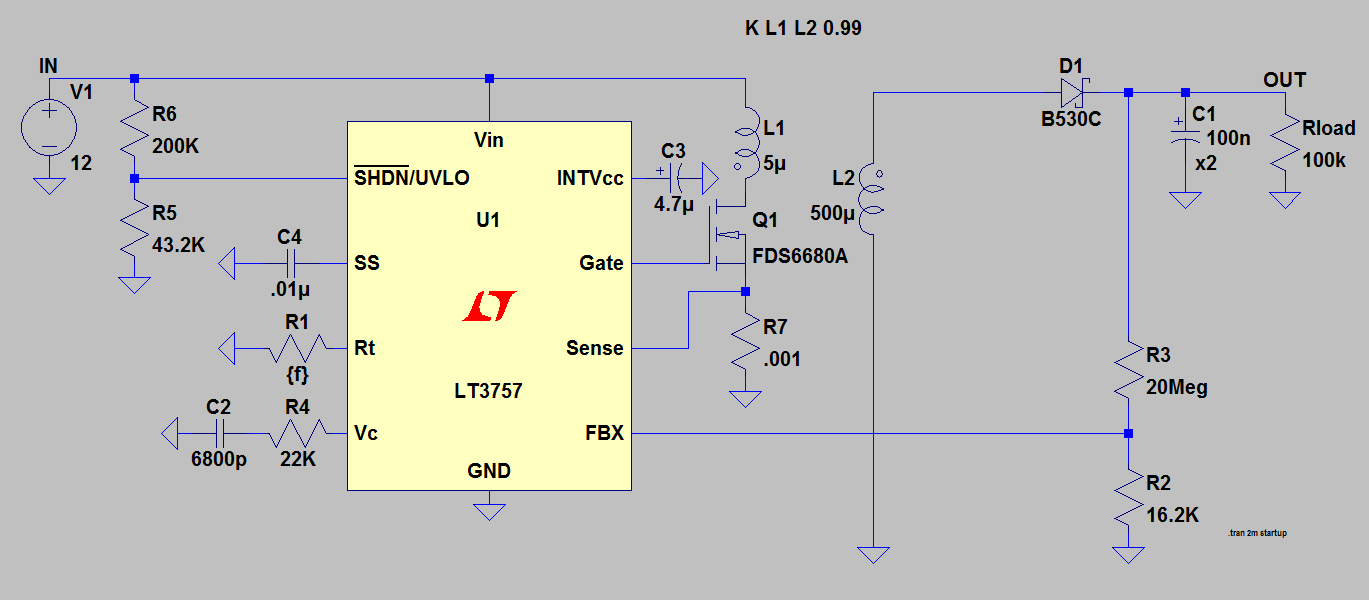
\includegraphics[width=1\columnwidth]{Slike/Simulacije/LM3757spice.png}
        \caption{\label{LM3757spice} Shema vezja v LTSpice.}
    \end{figure}
    
Problem pa nastane iz vidika varnosti, ker je sekundarno navitje visokonapetostnega transformatorja električno povezano z nizkonapetostno stranjo. Za zagotavljanje primerne izolacije bi moral napajalnik modula zdržati \SI{15}{\kilo\volt}, kar zopet pomeni načrtovanje takega napajalnika. Namreč napajalniki z najvišjo prebojno trdnostjo so takšni pod certifikatom IEC 60601-1 po katerem je najvišja prebojna trdnost \SI{4000}{\volt}AC.

	\subsubsection{LT8304} \label{LT8304}
LT8304 proizvajalca Linear Technology ~\cite{analog:LT8304} deluje po podobnem principu kot LM3748 z razliko, da ima vgrajen MOSFET in posledično manjšo izhodno moč. Simulacije so bile obetavne vendar sem jih vzel z rezervo, zaradi netočnosti modela transformatorja. Vseeno sem se odločil narediti prototipno ploščo s krmilnikom in pripadajočimi komponentami. Vezje je delovalo po pričakovanjih, vendar se je po približno 20 sekundah pokadilo iz krmilnika. Mislil sem, da je to bil samo problem z dotičnim krmilnikom in sem uporabil novega. Tudi pri temu se je pokadilo. Omenjen krmilnik ima maksimalno moč \SI{24}{\watt}, vendar pri meritvah moč ni presegla \SI{10}{\watt}. Potrebno se je pa zavedati, da je bil na izhodu napajalnika kondenzator s \SI{4700}{\micro\farad}, zaradi katerega napajalnik ni pokazal napetostnih špic, zaradi katerih je bila presežena izhodna moč. Drugi del, kjer bi lahko prihajalo do napake je na pinu SW, kateri je ponor internega MOSFETa. Lahko, da inducirana napetost na primarnem navitju je višja od \(U_{DS MAX}\) in posledično poškoduje čip. Podatkovni list narekuje uporabo Schottky in Zenner diode s pragovno napetostjo \(V_{Zenner(MAX)} \leq 145 V - V_{IN(MAX)}\) proti napajalni liniji za odvajanje prenapetostnih špic. V mojem primeru sem uporabil Zenner diodo s pragovno napetostjo \SI{100}{\volt}, vendar očitno ni bila dovolj. Imel sem še en krmilnik pri katerem sem namesto priporočene prenapetostne zaščite uporabil TVS diodo, z nominalno napetostjo \SI{70}{\volt} in maksimalnim tokom \SI{26.5}{\ampere}. Toda rezultat je bil še vedno isti.

    \subsubsection{Ugotovitve} \label{Ugotovitve glede komercialnih krmilnkov}
Po vseh simulacijah se je izkazalo, da ne bo mogoče uporabiti že narejenega krmilnika, vendar bo potrebno tudi krmilnik načrtovati od začetka. Možna rešitev je uporaba krmilnika LT3757, vendar namesto napajanja z omrežnim napajalnikom bi potrebno bilo uporabiti baterijsko napajanje. Baterije bi se polnile, ko je visokonapetostni napajalnik izklopljen, ob vklopu le-tega se baterije galvansko loči od polnilnika s pomočjo odklopnika kateri ima prebojno napetost vsaj \SI{15}{\kilo\volt}. Takšen odklopnik zopet pomeni nekaj zelo specifičnega in dragega ali pa samoizdelavo. 

	\subsubsection{Krmilnik z mikrokrmilnikom} \label{KrmilnikzUc}
Edina možnost, ki nam je še ostala je bila izdelava visokonapetostnega krmilnika z mikrokrmilnikom. Krmilnik bo opravljal le vlogo krmiljenja visokonapetostnega napajalnika. Vhodni signal bo prejel preko serijske povezave, povratna vezava bo pa preko analogno-digitalnega pretvornika, kateri bo na mikrokrmilnik povezan preko optičnega izolatorja za digitalne povezave.  Mikrokrmilnik je bil uporabljen STM32 iz družine F4, saj njegove operacije niso tako kritične in je lahko uporabljen praktično kateri koli mikrokrmilnik. Z STM Cube razvojim okoljem sem imel izkušnje že od prej, razvojna ploščica STM NUCLEO F4 je bila na zalogi v podjetju. Analogno-digitalni pretvornik tudi ni bil kritičen, saj za koncept nismo rabili neke visoke natančnosti, galvansko ločitev med visokonapetostnim in nizkonapetostnim delom je zagotavljal digitalni izolator z vgrajenim izolatorjem napajanja iz družine ISOW proizvajalca Texas Instruments. 

	\begin{figure}[H]
    \centering
    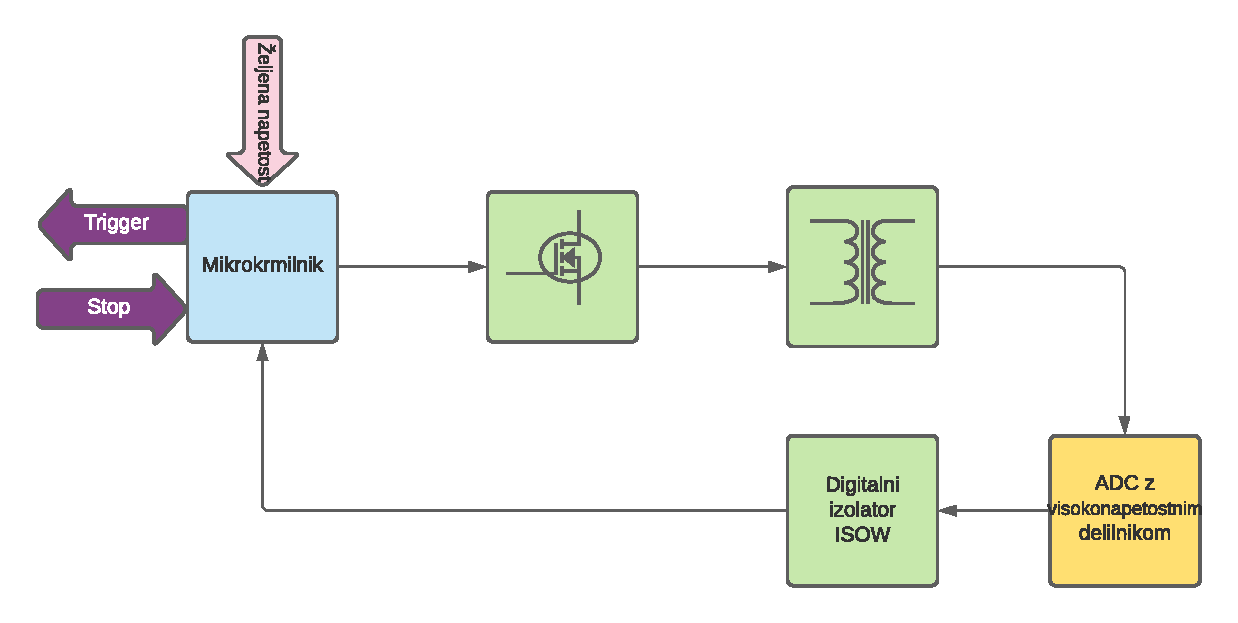
\includegraphics[width=1\columnwidth]{Sheme/KrmilnikzuCElShema.pdf}
    \caption{\label{KrmilnikzuCElShema} Shema visokonapetostnega krmilnika z mikrokrmilnikom.}
	\end{figure}

	\begin{figure}[H]
    \centering
    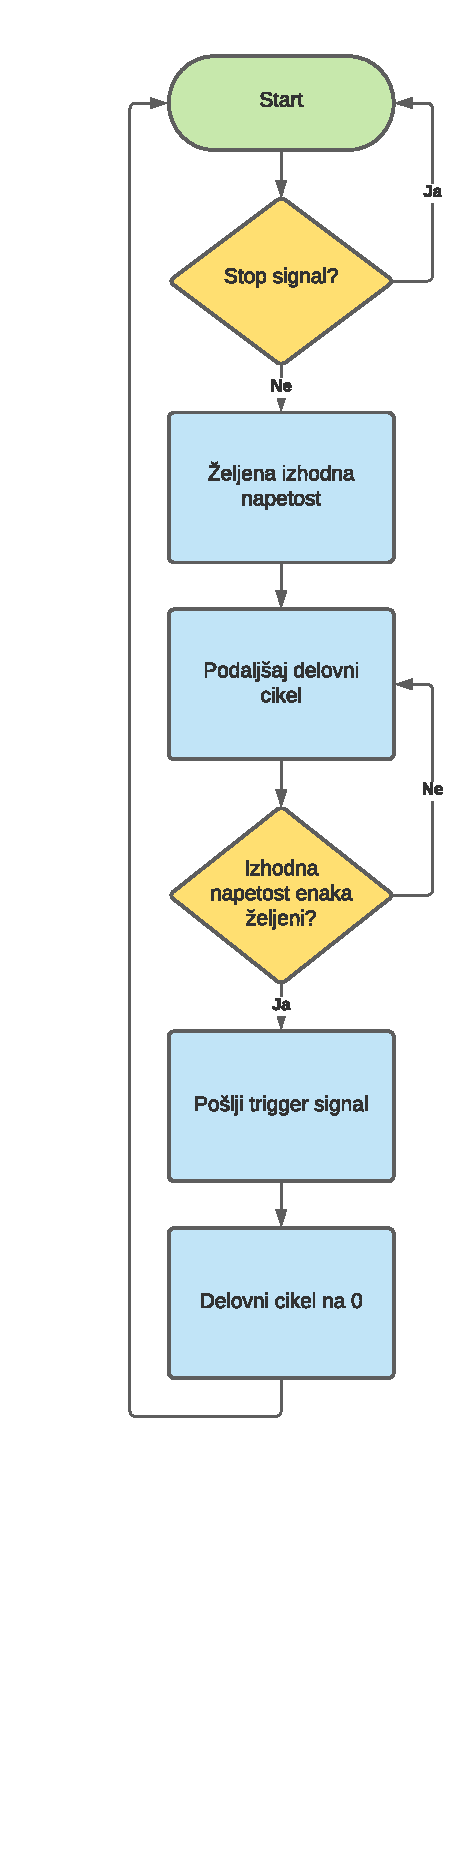
\includegraphics[width=0.35\columnwidth]{Sheme/KrmilnikzuCShema.pdf}
    \caption{\label{KrmilnikzuCShema} Shema programske kode visokonapetostnega krmilnika z mikrokrmilnikom.}
	\end{figure}
	
Programska koda preveri, če glavni krmilnik še pošilja STOP signal, če ga ne prebere željeno napetost preko serijske povezave in nastavi delovni cikel na najkrajšega. Dokler izhodna napetost ne doseže nastavljene, počasi povečuje delovni cikel. Ko izhodna napetost doseže nastavljeno, pošlje glavnemu krmilniku TRIGGER signal, se pravi signal kateri sproži praznilni rele in postavi delovni cikel na 0. Počasno dviganje napetosti nam omogoča počasnejše polnenje kondenzatorja in posledično potrebujemo manjši transformator. S tem krmilnikom sem uspel krmiliti izhodno napetost, bilo pa bi potrebno na fino nastaviti PID parametre.

	\subsection{Visokonapetostno stikalo} \label{Visokonapetostno stikalo}
	Standard zahteva ''bounce-less'' stikalo stikalo, katero ko sklene kontakt, ga ne razklene več. V preteklosti so se prodajali releji, kateri so imeli kontakte v kapsuli in notri malo živega srebra. Živo srebro je poskrbelo, da v času ko sta bila kontakta odbita je tok lahko še vedno tekel preko živega srebra. Vendar je zaradi direktive RoHS je izbira takšnih relejev zelo omejena.
	
	\subsubsection{Komercialno dobavljivi releji} \label{Komercialno dobavljivi releji}
     Prvotna izbira je bil model G61A proizvajalca Gigavac ~\cite{Gigavac:G61A}, kateri se tudi nahaja v simulatorjih elektrostatične razelektritve, saj je v specifikacijah poudarjeno: Odličen za praznjenje kondenzatorjev ter efektivno operira brez skakanja kontaktov.
    
    \begin{figure}[H]
        \centering
        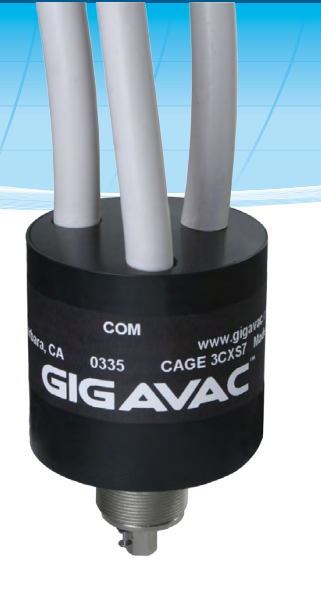
\includegraphics[width=0.5\columnwidth]{Slike/GigavacG61C.png}
        \caption{\label{GigavacG61C} Slika releja G61A proizvajalca Gigavac.}
    \end{figure}    
    
    Vendar se cena takšnega releja giba okoli 2000\euro{}. Zaradi omejenega proračuna ni bilo mogoče odobriti nakup dotičnega releja. Dobra alternativa se je zdel rele serije H proizvajalca Medler electronics ~\cite{Standex:H} (sedaj Standex electronics) kateri ima v specifikacijah navedeno ''Zamenjava za mokre releje z živim srebrom''. Pri ceni okoli 50\euro{} se je to zdelo predobro, da bi bilo res.
    
    \begin{figure}[h]
        \centering
        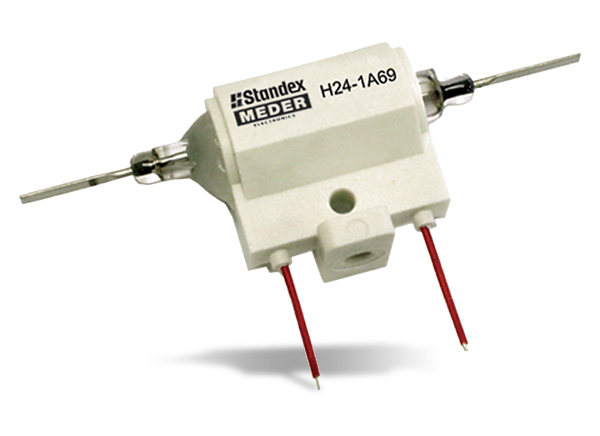
\includegraphics[width=1\columnwidth]{Slike/MederReleH.png}
        \caption{\label{MederReleH} Slika releja serije H proizvajalca Meder.}
    \end{figure}        
    
    
    Testi so pokazali točno to, kar smo pričakovali: skakanje kontaktov.
    
    \begin{figure}[H]
    \centering
        \begin{circuitikz}
           \draw (2,1)
            to[V, v=$Sig$] (2,3)
            to[short] (4,3)
            to[L] (4,1)
            to[short] (2,1);
        
           \draw (0,0)
            to[short] (0,1)
            to[C=10 nF] (0,3)
            to[short] (0,4)
            to[R=10 Ohm] (5,4)
            to[normal open switch] (5,0)
            to[short] (0,0);
    
        \draw (2.5,6) node[oscopeshape](osc1){}
        (osc1.left) node[anchor=west] {}
        (osc1.right) node[anchor=east] {};
        
        \draw (osc1.left)
        to[short] (0,6)
        to[short] (0,4);
        
        \draw (osc1.right)
        to[short] (5,6)
        to[short] (5,4);
        
        \draw (0,4) node[circ]{};
        \draw (5,4) node[circ]{};
	\end{circuitikz}
	   \caption{\label{MerilnoVezjeRele} Shema vezja za merjenje relejev.}
    \end{figure}
    
    \begin{figure}[H]
        \centering
        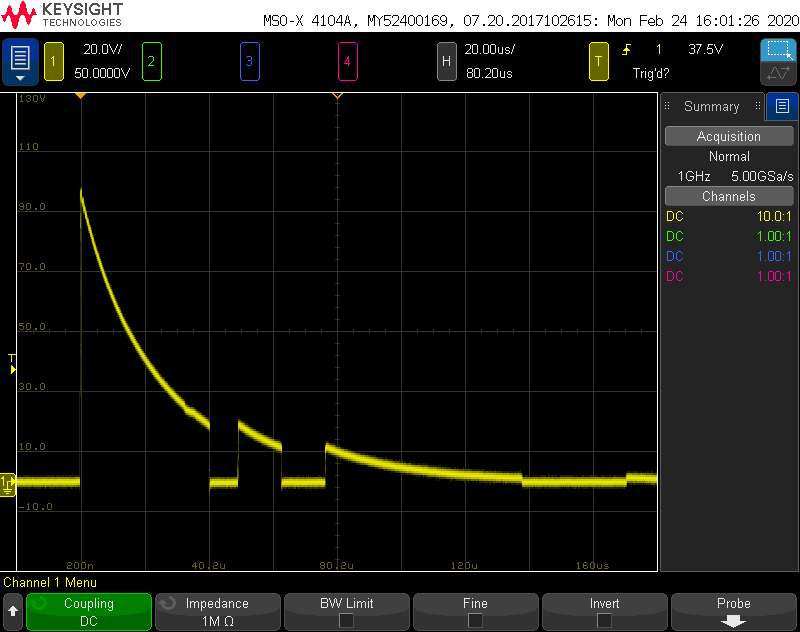
\includegraphics[width=1\columnwidth]{Slike/MedlerElectronicsRele.png}
        \caption{\label{BlokDiagramShema} Skakanje kontaktov pri releju proizvajalca Medler electronics.}
    \end{figure}
    
    ~\\Po specifikacijah bo največji tok čez rele \SI{10}{\ampere}, saj imamo maksimalno napetost \SI{15}{\kilo\volt} in kondenzator praznimo z \SI{1500}{\ohm} uporom. Zaradi varnosti sem pri merjenju spremenil RC konstanto iz \SI{1500}{\ohm} in \SI{100}{\pico\farad} na \SI{10}{\ohm} in \SI{10}{\nano\farad} katero sem napajal iz \SI{100}{\volt}. Na posnetku zaslona iz osciloskopa se lepo vidi razklenitev pri \SI{40}{\micro\second} in \SI{55}{\micro\second}. Po ponovitvah sem ugotovil, da so razklenitve časovno zelo konstantne. Nastala je ideja o vezanju dveh ali več enakih relejev vzporedno in vzbujanje le teh s časovnim zamikom, saj bi tako premostili razklenitev. Vendar bi s tem dodali kapacitivnost v sistem na katero moramo biti zelo pozorni saj standard dovoljuje maksimalno \SI{20}{\nano\second} odstopanja časovne konstante.
    Iz radovednosti sem naredil meritve še pri višjih napajalnih napetostih vzbujevalne tuljave, kjer sem predpostavljal, da bo magnetno polje dovolj močno, da se kontakt ne bo uspel odbiti. Vendar temu ni bilo tako saj so se prekinitve še vedno dogajale tudi pri trojni napajalni napetosti.
   
	\subsubsection{Komercialna tranzistorska rešitev} \label{Komercialna tranzistorska rešitev}   
    
	Mojo pozornost je pritegnil tudi izdelek podjetja Behlke, katero se ukvarja z visokonapetostno in močnostno elektroniko. Izdelek je bil HTS 181-02-C ~\cite{Behlke:HTS181-02-C} hitro visokonapetostno tranzistorsko stikalo. Dotični model ima maksimalno napetost \SI{18}{\kilo\volt} ter maksimalno tokovno špico \SI{12}{\ampere}. Malo manj vzpodbudne so številke za čas naraščanja saj bi v naših primerih bile od \SI{12}{\nano\second} do \SI{25}{\nano\second}. Kar je precej več kot \SI{10}{\nano\second} kot jih zahteva standard. Cena takega stikala je okoli 1100\euro , tako da zopet presega naš proračun. Vendar sem našel sliko odprtega stikala, kar mi je porodilo idejo o samo-izdelavi tranzistorskega visokonapetostnega stikala.
	
	\subsubsection{Samogradnja tranzistorskega visokonapetostnega stikala} \label{Samogradnja tranzistorskega visokonapetostnega stikala}
	
	Pozorno opazovanje slik visokonapetostnih stikal proizvajalca Behlke je prineslo ugotovitve, da je stikalo sestavljeno iz dveh delov: krmilni del in visokonapetostni del. Krmilni del ni zanimiv, vendar visokonapetostni je zelo, saj se vidi kako je zaporedno nanizanih okoli 10 tranzistorjev. Če predpostavimo, da imajo vsi tranzistorji enake karakteristike in se v istem času začnejo odpirati, bo napetost naraščala na vseh enako in skupni dvižni čas bo enak dvižnemu času tranzistorja. Prva ovira je bila izbiraje polprevodnikov, kateri so primerni za nalogo. IGBTji IXYL60N450 ~\cite{IXYS:IXYL60N450} proizvajalca LittleFuse so se na papirju izkazali za najboljše, saj imajo maksimalno \(V_{CES}\) napetost \SI{4.5}{\kilo\volt}, vendar imajo tipični odpiralni čas \SI{55}{\nano\second}, kar je še vedno 5.5 krat preveč. 

    Sem pa našel tranzistorje kateri so bili namenjeni za \SI{10}{\kilo\volt} z dvižnim časom okoli \SI{10}{\nano\second}. Tako bi lahko uporabili dva in ju zbondirali na tiskano vezje in s tem zmanjšali parazitne kapacitivnosti in induktivnosti. Vendar zaradi tako hitrega dvižnega časa spadajo ti tranzistorji pod ''izdelke z dvojnim namenom'' in za nakup le teh potrebno podpisati pogodbo o nerazkritju informacij.
Vendar mi je dalo misliti, če se uporabi najbolj idealne komercialne tranzistorje, jih odstrani iz ohišja in zbondira na tiskano vezje. S tem bi lahko dosegli najnižje vrednosti parazitnih kapacitivnosti in induktivnosti. Preden začnem risati tiskano vezje sem hotel v simulatorju zasnovati še krmilnik. Uporabljeni bi bili IGBTji zato je potrebno krmilno napetost pripeljati med vrata in emitor. V mojem primeru je potencial emitorja najvišjega IGBTja proti masi \SI{11.25}{\kilo\volt}. S primernimi visokonapetostnimi stikali bi lahko krmilil na način s preklopi kondenzatorja t.i. ''Switched Cap''.

    %shema swtiched cap
    \begin{figure}[H]
    \centering
        \begin{circuitikz}
            \draw (0,0)
            to[V, v=$Sig$] (0,3)
            to [short] (1.185,3)
            to[short] (1.185,2.85);
            
            \draw (1.5,2.3)
            node[spdt, rotate=90] (sw1) {}
            (sw1.in) node[left] {};
            
            \draw (1.5,0.7)
            node[spdt, rotate=-90, yscale=-1] (sw2) {}
            (sw2.in) node[left] {};;
             
            \draw (sw1.in)
            to[C] (sw2.in);
           
            \draw  (1.815,0.15)
            to[short] (1.815,0)
            to[short] (4,0)
            to[short] (4,1.5);
            
            \draw (4,2)
		node[nigfetd](Q){}
		(Q.G) node[left] {};
		
		\draw (Q.G) to[short] (3.0145,3)
		to[short] (1.815,3)
		to[short] (1.815, 2.85);
		
		\draw (0,0)
            to[short] (1.185, 0)
            to[short] (1.185, 0.15);    
        \end{circuitikz}
                \caption{\label{SwitchedCapFetDriver} Shema idejne zasnove krmiljenja tranzistorja preko ''Switched Cap''.}
    \end{figure}
    Naletel sem pa na članek \cite{doi:10.1063/1.1143294}, kjer so potrebovali podobno rešitev, ki so jo reševali z transformatorji kateri so imeli 1:1 razmerje in primerno prebojno trdnost. V simulacijah se je rešitev obnesla. V resničnem svetu bi me pa skrbelo, če bi kakšen krmilnik ali tranzistor le malo zakasnil, saj bi takrat pristala celotna napetost na njemu, kar bi seveda pomenilo preobremenitev le tega.
    
	\subsubsection{Mehanska rešitev} \label{Mehanska rešitev}    
    
    
    V iskanju nadaljnjih rešitev to pomeni mehanično rešitev in samo eno stikalo ne zaporedne ali vzporedne vezave stikal. Lotili smo se hitrih prototipov štirih stikal:
    \begin{enumerate}
   
        \item  Solenoid, kateri drži razklenjena kontakta, skupaj ju vleče vzmet. Ob sprožitvi se obrne polariteta napajanja tuljave solenoida, kateri poleg vzmeti tišči kontakta skupaj.
    \begin{figure}[H]
        \centering
        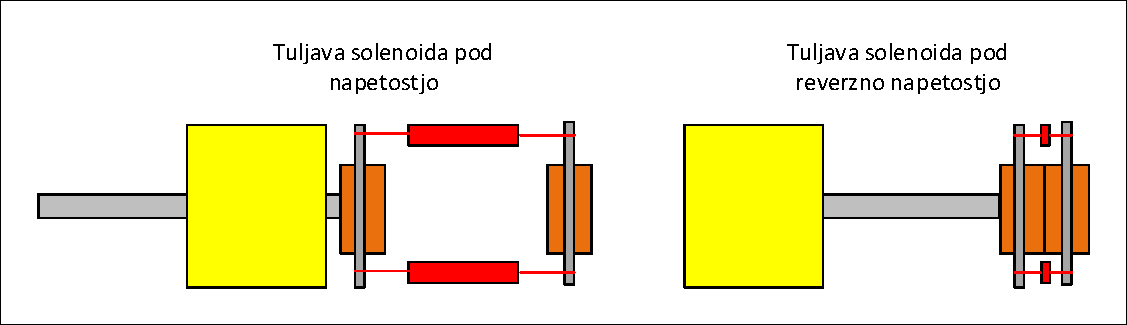
\includegraphics[width=1\columnwidth]{Sheme/StikaloSolenoidVerzija1.pdf}
        \caption{\label{/StikaloSolenoidVerzija1} Shema stikala s solenoidom verzija 1.}
    \end{figure}
    
    \item  Solenoid kateri porine kontakt in ga jezička ujameta.
    \begin{figure}[H]
        \centering
        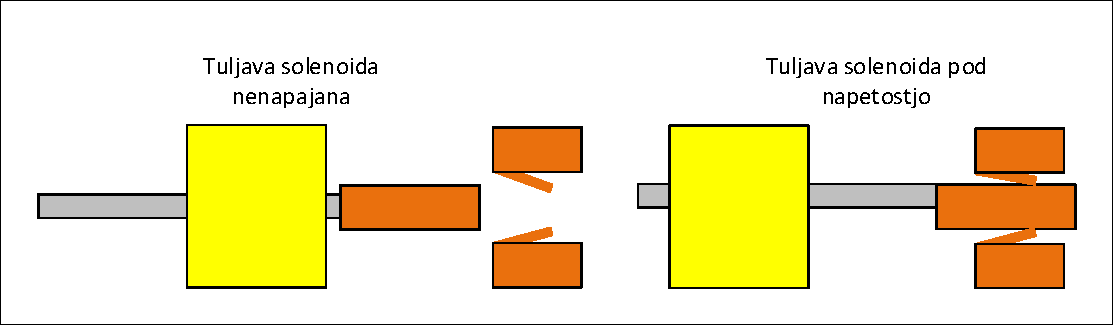
\includegraphics[width=1\columnwidth]{Sheme/StikaloSolenoidVerzija2.pdf}
        \caption{\label{/StikaloSolenoidVerzija2} Shema stikala s solenoidom verzija 2.}
    \end{figure}
    
    \item  Servo motor se zasuče in z drsnim stikalom sklene kontakt.
    \begin{figure}[H]
        \centering
        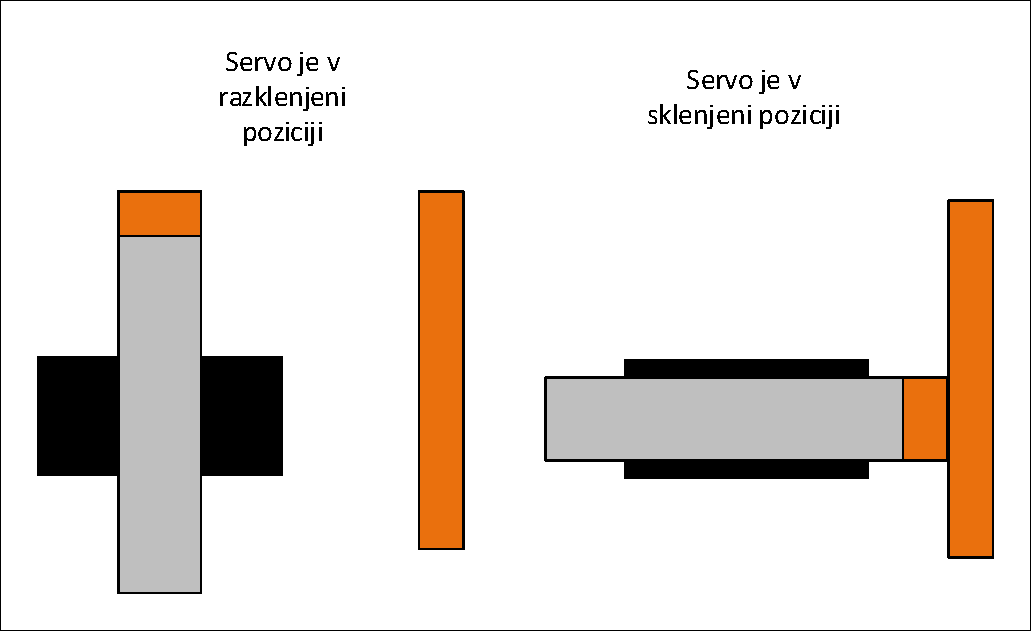
\includegraphics[width=1\columnwidth]{Sheme/StikaloServoVerzija1.pdf}
        \caption{\label{StikaloServoVerzija1} Shema stikala s servo motorjem verzija 1.}
    \end{figure}
    
    \item  Servo motor se zasuče in pritisne na kontakt kateri je na vzmeti.
    \begin{figure}[H]
        \centering
        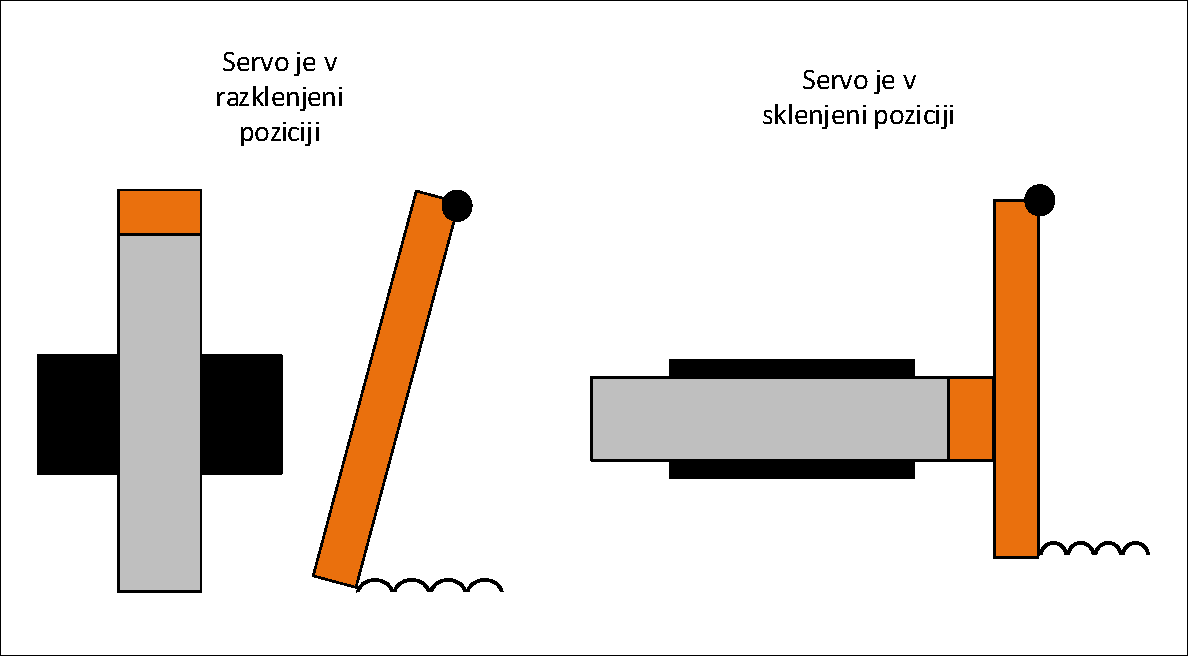
\includegraphics[width=1\columnwidth]{Sheme/StikaloServoVerzija2.pdf}
        \caption{\label{StikaloServoVerzija2} Shema stikala s servo motorjem verzija 2.}
    \end{figure}
\end{enumerate}


    ~\\Za solenoid smo na začetku uporabili manjši model, kateri je bil namenjen konstantnemu delovanju pri \SI{12}{\volt}, za hitrejše delovanje in večjo silo se ga lahko prenapaja z  \SI{40}{\volt} za čas  \SI{1}{\second} z delovnim ciklom 5\%. Izkazal se je za neuporabnega, saj čim se na njega namesti kontakt, nima več zadostne moči za premikanje, posebno če bi se moral še upirati sili vzmeti. Za hitri preizkus mojih tez sem naredil solenoid na tuljavniku od transformatorja.
    %probat še z močnejšim solenoidom
    
    ~\\S stikalom s servo motorjem smo imeli dokaj dobre uspehe, vendar smo še vedno bili daleč od končne rešitve. Hitre meritve prototipa stikala z servo motorjem verzija 1, so pokazale dvižni čas  \SI{10}{\nano\second} kjer se vseeno pojavljajo manjše prekinitve po sklenitvi kontaktov. Skrbi me pa tudi obraba in oksidacija kontaktov. Rešitev bi bila zaprtje celotnega stikala v vakuumsko komoro ali še bolje v plin $SF_{6}$ kateri ima zelo visoko prebojno trdnost.
    
    \begin{figure}[H]
        \centering
        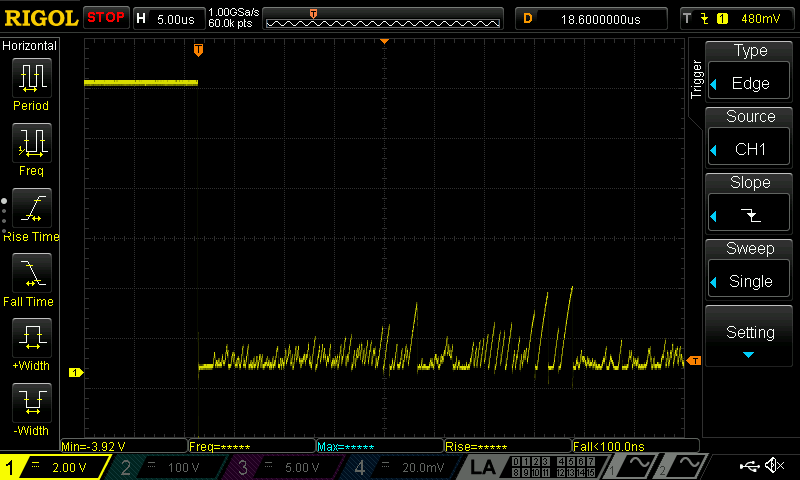
\includegraphics[width=1\columnwidth]{Slike/ServoStikalo1/ServoStikalo1.png}
        \caption{\label{ServoStikalo1} Potek napetosti po sklenitvi kontaktov pri servo stikalu verzija 1.}
    \end{figure}
    
    \begin{figure}[H]
        \centering
        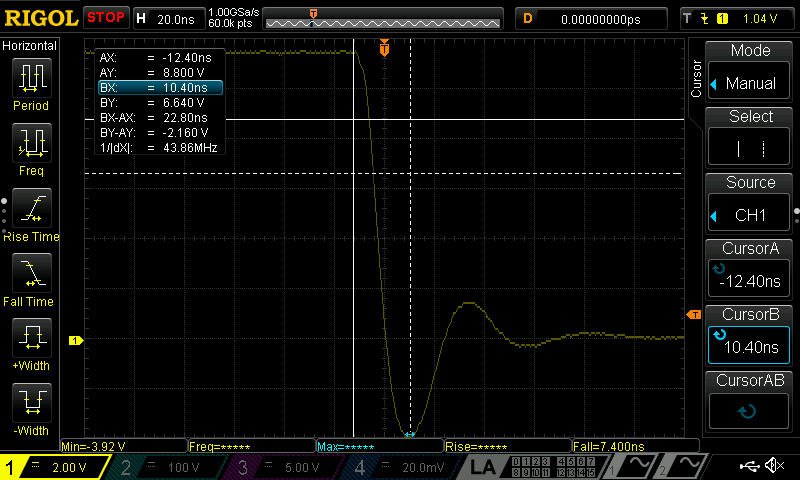
\includegraphics[width=1\columnwidth]{Slike/ServoStikalo1/ServoStikalo1povecano.png}
        \caption{\label{ServoStikalo1povecano} Potek napetosti po sklenitvi kontaktov pri servo stikalu verzija 1 povečano.}
    \end{figure}
    
    ~\\Stikalo s servo motorjem verzija 2 pa je problem počasnega dvižnega časa. Verjetno je kriva vsa parazitna kapacitivnost. Potrebno bi bilo narediti revizijo in skrajšati vse segmente žice in narediti kontakte bolj kompaktne. 
    





\chapter{Sklep} \label{Sklep}

	Kljub temu, da se je že ob zasnovi projekta vedelo, da bo celoten projekt izjemno težavno izpeljati v predlaganem časovnem okvirju in proračunu, nismo pričakovali takšnih zapletov. Večji del problemov je predstavljala zahtevana visoka napetost, saj se komercialno dobavljive komponente dobijo do okoli \SI{3}{\kilo\volt}, za višje napetosti pa postanejo komponente že težje dobavljive in posledično dražje. Ogromno preglavic je povzročal tudi rele brez skakanja, saj se načeloma uporabljajo za nizke napetosti. Poleg tega vsebujejo nevarne substance, kar jih naredi še bolj redke. Kljub temu sem z ugotovitvami prišel do kar nekaj uporabnih rešitev, katere bom še bolj raziskal pri izdelavi diplomske naloge. Do delujočega ESD simulatorja bi lahko prišel z uporabo komercialnega visokonapetostnega nastavljivega napajalnika proizvajalca Applied Kilovolts in visokonapetostnim relejem namenjenim praznjenju kapacitivnih zalogovnikov proizvajalca Gigavac, vendar bi taka rešitev podražila projekt za vsaj 5000\texteuro. Druga možnost je lastni razvoj visokonapetostnega nastavljivega napajalnika in visokonapetostnega releja, katera bi približno enako podražila projekt toda bi bilo potrebnih 400 delovnih ur več. V podjetju pa tudi nimamo izkušenj s tako visokimi napetostmi, saj se ukvarjamo z mikroelektroniko.
	
	
	
\bibliographystyle{acm}	
\bibliography{literatura} 




\end{document}
%%%%%%%%%%%%%%%%%%%%%%%%%%%%%%%%%%%%%%%%%%%%%%%%%%%%%%%%%%%%%%%%%%%%%%%%%%%%%%%%%%%%%%%%%%%%%%%%%%%%%%%%%%%%%%%%%%%%%%%%
